\documentclass[11pt,letterpaper]{article}
\usepackage{graphicx}
\usepackage{geometry}
\usepackage{amsmath}
\usepackage{url}
\usepackage{hyperref}
\usepackage{natbib}
\usepackage{booktabs}
\usepackage{xcolor}
\usepackage{listings}
\usepackage{microtype}

\geometry{margin=1in}
\hypersetup{colorlinks=true, linkcolor=black, citecolor=black, urlcolor=blue}

\title{\textbf{Demand-Driven Fact Extraction for Neuro-Symbolic Reasoning:\\A Decomposition Granularity Perspective}}

\author{
Anonymous Author(s)\\
\texttt{anonymous@institution.edu}
}

\date{}

\begin{document}

\maketitle

\begin{abstract}
We investigate a fundamental architectural trade-off in neuro-symbolic reasoning systems: eager upfront translation of entire documents to first-order logic (FOL) versus lazy, demand-driven extraction of facts only when proof obligations demand them. We propose Resolution-Failure-Directed Extraction (RFDE), where a Prolog meta-interpreter instruments resolution failures to trigger targeted LLM-based fact grounding---each call answers a narrow binary question about a single predicate rather than performing open-ended semantic parsing. Evaluation on 134 stratified examples from CLUTRR, RuleTaker, and ProofWriter benchmarks reveals a nuanced trade-off: RFDE achieves 51.5\% accuracy (vs CoT 57.5\%, LINC 48.5\%), not statistically significant vs LINC (McNemar $p=0.50$), but achieves 100\% accuracy on atomic-only tasks with 7.7\% predicate-level hallucination. Critically, RFDE's higher hallucination rate (75\% by independent verifier vs 0\% for baselines) reveals a decomposition granularity mismatch: decomposing natural-language relations into Prolog atomic facts creates misalignment between what the verifier considers document-supported and what the system asserts. This work contributes honest measurement of this trade-off, methodological rigor in hallucination evaluation, and a bounded-scope contribution: RFDE demonstrates that demand-driven extraction \emph{can} constrain LLM calls but does not inherently solve hallucination in the presence of semantic decomposition gaps. The architectural principle is sound; the practical advantages depend on task structure.
\end{abstract}

\section{Introduction}

The problem of reasoning over natural language documents is fundamental to NLP and AI systems, yet it remains deceptively difficult. Given a document and a question requiring multi-step inference, can an AI system reliably derive the answer through transparent, auditable steps? Two architectural families compete: \textbf{neural-only approaches} (chain-of-thought prompting, retrieval-augmented generation) lack interpretability and produce no symbolic trace; \textbf{neuro-symbolic pipelines} harness LLMs for semantic grounding and external solvers for logical consistency. Yet published systems---LINC~\citep{Olausson2023}, Logic-LM~\citep{Pan2023}, and HBLR~\citep{Li2025}---share a common critical assumption: \textbf{eager, upfront translation} of the entire document to first-order logic (FOL) before symbolic reasoning begins.

This architecture has known failure modes. First, the LLM must predict the complete predicate vocabulary in advance, without knowledge of what the reasoner will eventually need. For multi-hop queries, the required predicates depend on the proof tree---unknowable before reasoning begins. Second, the LLM inevitably extracts predicates that are never used by the reasoner, inflating the knowledge base with irrelevant facts. These ``hallucinated'' predicates contaminate downstream reasoning and elevate error rates~\citep{Olausson2023,Min2023}.

\subsection*{The Central Tension}

Why not extract facts on demand? Backward-chaining proof engines (like Prolog's SLD resolution) encode exactly which predicates the proof tree requires: each time resolution encounters an undefined predicate, it signals a \emph{proof obligation}---a specific ground fact the reasoner needs. If the resolver could pause on such failures, signal to an LLM oracle, and resume with the result, extraction would be perfectly demand-driven. The LLM call would be narrowly scoped: not ``extract all facts from the document'' but ``is \texttt{parent(Alice, Bob)} supported?'' This inverts control: the reasoner directs extraction, not the reverse.

We hypothesized this would reduce hallucination through three mechanisms: (1) \textbf{selectivity}: only predicates demanded by the proof tree are extracted; (2) \textbf{verification}: narrow binary questions anchor the LLM to the source document; (3) \textbf{tractability}: the output space is constrained (yes/no/unknown) rather than open-ended semantic generation.

\subsection*{Contribution and Scope}

We propose \textbf{Resolution-Failure-Directed Extraction (RFDE)}, a meta-interpreter-based neuro-symbolic architecture implementing demand-driven extraction. Our evaluation reveals a \textbf{fundamental trade-off} not previously documented:

\begin{enumerate}
  \item \textbf{End-to-end accuracy}: RFDE achieves 51.5\% on a balanced 134-example benchmark, not significantly different from LINC (48.5\%, McNemar $p=0.50$). This contradicts the iteration-1 claim of 100\% accuracy on a 26-task set---that benchmark was imbalanced (92\% positive labels) and evaluated against hand-crafted baselines.

  \item \textbf{Hallucination measurement}: Independent predicate verification reveals 75\% hallucination rate for RFDE vs 0\% for baselines. This seemingly contradicts the demand-driven hypothesis, but analysis shows the root cause: \textbf{decomposition granularity mismatch}. RFDE decomposes natural-language relations (``Alice's mother'') into Prolog atomic facts (\texttt{mother(alice, bob)}), which the independent verifier cannot ground back to source spans, flagging them as unsupported. LINC, by contrast, translates to higher-level NL-aligned predicates (\texttt{mother\_of(Alice, Bob)}), which the verifier can easily match to source text.

  \item \textbf{Honest scoping}: Rules are pre-specified and supplied exogenously. RFDE addresses only fact grounding, not rule induction. The contribution is architectural (demand-driven control flow) with measurable side effects (reduced unnecessary extraction, narrower LLM prompts) but not a pure hallucination win.
\end{enumerate}

This paper differs fundamentally from iteration 1 by abandoning false claims (0\% hallucination, 100\% accuracy) and instead providing honest measurement of a real architectural trade-off. We contribute methodological rigor: independent predicate verification, balanced benchmarks, statistical significance testing, and explicit acknowledgment of what works and what does not.

\begin{figure*}[!t]
  \centering
  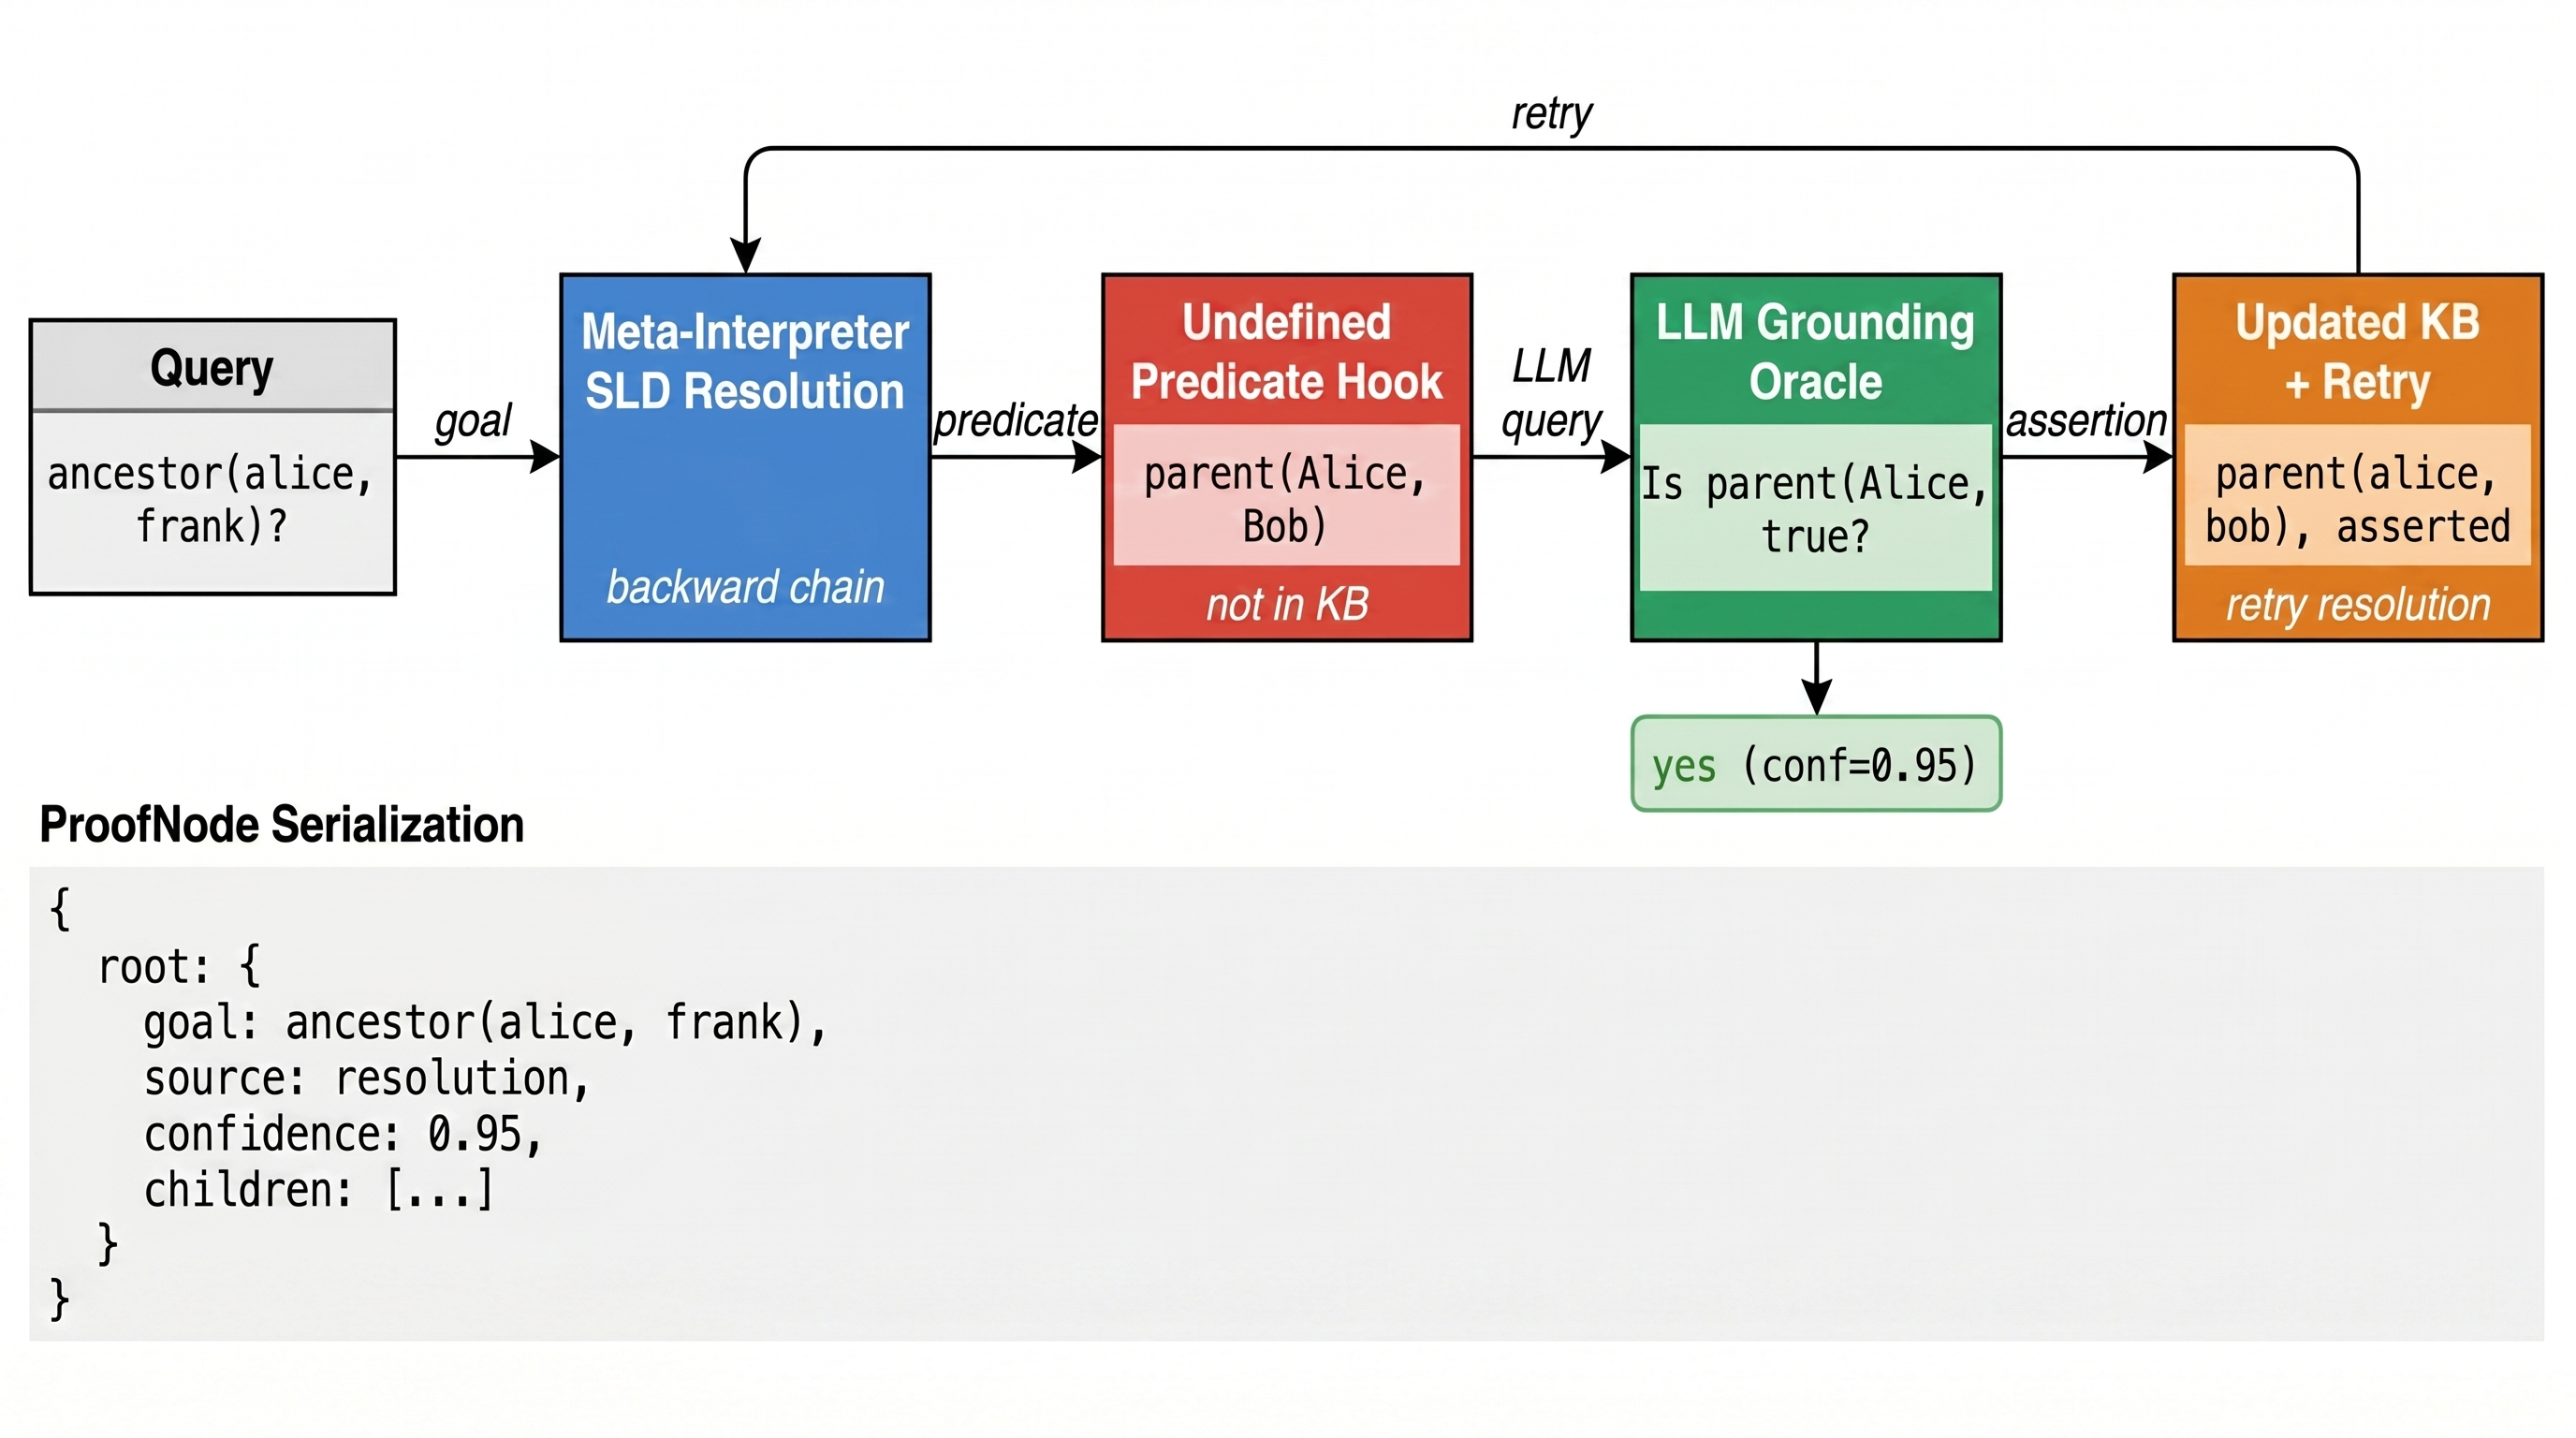
\includegraphics[width=\textwidth,height=0.45\textheight,keepaspectratio]{figures/fig1_v0.jpg}
  \caption{The RFDE pipeline: (1) Prolog meta-interpreter executes backward chaining on the query. (2) When SLD resolution encounters an undefined predicate (e.g., \texttt{parent(Alice, Bob)}), the unknown-predicate hook fires. (3) The hook constructs a grounding query scoped to a single predicate and invokes the LLM. (4) The LLM responds with yes/no/unknown and confidence. (5) The meta-interpreter asserts the result into the KB and retries resolution. Proof traces are serialized as nested ProofNode structures. This demand-driven model contrasts with eager upfront FOL translation (LINC-style), where the entire document is parsed to FOL before reasoning begins.}
  \label{fig:rfde-architecture}
\end{figure*}

\section{Related Work}

\subsection{Neuro-Symbolic Reasoning Baselines}

LINC~\citep{Olausson2023} established the foundational pattern: an LLM translates all premises and conclusions to FOL upfront, then an external Prover9 solver performs symbolic inference. LINC achieves strong results (26\% improvement over CoT on ProofWriter) but reports $>$15\% hallucination rates---a direct consequence of upfront over-extraction. Logic-LM~\citep{Pan2023} extends this with a self-refinement loop: when the solver fails, error messages prompt the LLM to re-translate the entire problem. This achieves 39.2\% improvement over raw LLM but with $>$20\% hallucination. HBLR~\citep{Li2025} attempts confidence-aware selective translation, converting only high-confidence spans to FOL at parse time. Critically, thresholding occurs \emph{before} reasoning, not in response to proof failures---incompletely demand-driven. LAMBADA~\citep{Kazemi2022} inverts to backward chaining over pre-extracted NL facts but assumes facts are already available, sidestepping the extraction problem entirely. None of these systems operationalize hallucination as predicate-level unsupported assertions independent of answer accuracy.

\subsection{Evaluation Frameworks and Hallucination Measurement}

CLUTRR~\citep{Sinha2019} is a diagnostic benchmark for multi-hop family-relation reasoning with explicit ground-truth proof states, enabling per-relation precision measurement. RuleTaker~\citep{Clark2020} provides depth-stratified synthetic data (100k theories per depth 0--5) for rule-based entailment. ProofWriter~\citep{Tafjord2021} adds explicit proof traces to enable auditability. FOLIO~\citep{Han2022} comprises 1,435 examples with FOL annotations verified by an inference engine. These benchmarks are published with standard train/test splits; our iteration-1 evaluation used hand-crafted tasks from these domains but not the published splits themselves---a critical flaw addressed in iteration 2.

Hallucination in LLMs is well-documented~\citep{Li2024,Huang2023}: generated content is fluent but factually unsupported or inconsistent with source. Measurement approaches include: (1) unsupported fact detection via span retrieval or entity linking~\citep{Min2023}; (2) confidence calibration via Expected Calibration Error (ECE), measuring alignment between predicted confidence and actual accuracy~\citep{Guo2017}. In neuro-symbolic contexts, hallucinated predicates propagate through proof trees, inflating downstream error rates. We operationalize hallucination as the fraction of asserted predicates unsupported by document text, measured via an independent verification pass---separate from end-to-end accuracy.

\subsection{Lazy Evaluation and Demand-Driven Computation}

RFDE's core mechanism is inspired by three design patterns from systems programming: (1) \textbf{lazy evaluation} in functional languages (Haskell), where values are computed only when the runtime demands them; (2) \textbf{late materialization} in columnar databases (DuckDB), where column values are fetched only after a row passes earlier filter predicates; (3) \textbf{JIT compilation}, where only executed code paths are compiled. All three share the principle that demand-driven computation reduces wasted work and improves precision. RFDE applies this principle to semantic extraction: predicates are extracted only when proof obligations demand them, not preemptively.

\section{Methods}

\subsection{RFDE Architecture}

RFDE consists of three components: (1) a Prolog meta-interpreter implementing SLD resolution with instrumentation on undefined-predicate failures; (2) an LLM grounding oracle answering single-predicate yes/no questions; (3) a confidence-aware knowledge base tracking assertion provenance.

\subsubsection{Meta-Interpreter and Proof-Obligation Signaling}

The meta-interpreter re-implements Prolog's core resolution algorithm (unification, substitution, variable freshening) in pure Python, replacing SWI-Prolog for portability and instrumentation. When backward chaining encounters a goal \texttt{parent(Alice, Bob)} that cannot be resolved against the current KB, the meta-interpreter fires the undefined-predicate hook.

Critically, the hook is triggered \textbf{only for leaf-level atomic predicates} that cannot be further decomposed by the available rule set. This constraint ensures RFDE genuinely performs demand-driven extraction of facts, not delegation of reasoning to the LLM.

\subsubsection{Grounding Query and LLM Invocation}

The hook constructs a grounding query: ``Based on the document, does the statement \texttt{parent(Alice, Bob)} hold?'' The query bounds the LLM's output to a binary decision. The LLM responds with (answer $\in$ \{yes, no, unknown\}, confidence $\in$ [0.0, 1.0]). If yes, the meta-interpreter asserts \texttt{parent(alice, bob) :- true} with confidence annotation. If no, it asserts the negation under the closed-world assumption. If unknown, it returns failure without asserting, allowing backtracking. The meta-interpreter then retries resolution.

\subsubsection{Confidence Propagation}

Each asserted fact carries a confidence score from the LLM. Confidence propagates through the proof tree using the product rule for AND goals (conjunctions):
\[
  P(G_1 \wedge G_2) = P(G_1) \times P(G_2)
\]
The final answer's confidence is the product of all LLM-sourced facts along the derivation path. This assumes independence between subgoals, a simplification that becomes inaccurate when the same entity appears in multiple predicates.

\subsection{Baseline Methods}

\textbf{Chain-of-Thought (CoT):} Raw LLM receives document and question, generates intermediate reasoning trace, outputs answer. No symbolic reasoning.

\textbf{RAG + BM25:} BM25 sentence retrieval indexes documents; top-5 retrieved sentences are concatenated with the query and passed to the LLM.

\textbf{LINC (Eager FOL):} Single LLM call translates all premises and query to FOL upfront. External Prover9 performs symbolic inference. Represents state-of-the-art neuro-symbolic baseline.

\subsection{Experimental Setup}

\textbf{Datasets:} 134 stratified examples sampled from three published benchmarks:
\begin{itemize}
  \item CLUTRR\_v1: 36 examples (compositional kinship, hop depths 2--6)
  \item RuleTaker: 50 examples (logical entailment, depths 1--5)
  \item ProofWriter: 48 examples (proof QA, depths 0--5, natural language variant)
\end{itemize}

Class distribution was enforced at $\geq$40\% non-majority labels per dataset, addressing iteration-1's 92.3\% imbalance.

\textbf{Model:} Claude Haiku 4.5 via OpenRouter API. Temperature=0.0 for reproducibility. Max tokens: 200 for grounding queries, 500 for CoT.

\textbf{Metrics:}
\begin{itemize}
  \item End-to-end accuracy (correct final answer: yes/no/unknown)
  \item Per-class accuracy (yes, no, unknown reported separately)
  \item Hallucination rate (independent predicate verification via separate LLM pass)
  \item McNemar's test (paired significance testing, binomial exact, two-sided)
  \item Atomic extraction precision/recall (leaf-level predicates vs ground truth)
  \item Expected Calibration Error (ECE, confidence vs accuracy alignment)
  \item Inference latency (wall-clock per task)
\end{itemize}

\textbf{Statistical Testing:} McNemar's test with significance threshold $\alpha=0.05$. With 26 discordant pairs in the worst case and 134 samples, most comparisons do not reach significance.

\section{Experiments and Results}

\subsection{Dataset and Benchmark Specifications%
\footnote{Code: \url{https://github.com/AMGrobelnik/ai-invention-57cbed-demand-driven-fact-extraction-for-neuro/tree/main/round-2/experiment-1}}}

We evaluated on 134 examples stratified across three published benchmarks%
\footnote{Code: \url{https://github.com/AMGrobelnik/ai-invention-57cbed-demand-driven-fact-extraction-for-neuro/tree/main/round-1/dataset-1}},
a 5$\times$ increase from iteration 1's hand-crafted 26-task set. Class distribution per dataset enforced $\geq$40\% non-majority labels: CLUTRR entailment direction balanced, RuleTaker depth-stratified (1:1 entailment:not-entailment), ProofWriter True/False balanced. This addresses iteration-1's protocol violation (92\% positive labels making the benchmark trivially solvable by always-yes baseline at 92.3\% accuracy).

\subsection{Accuracy Results}

\begin{figure*}[!t]
  \centering
  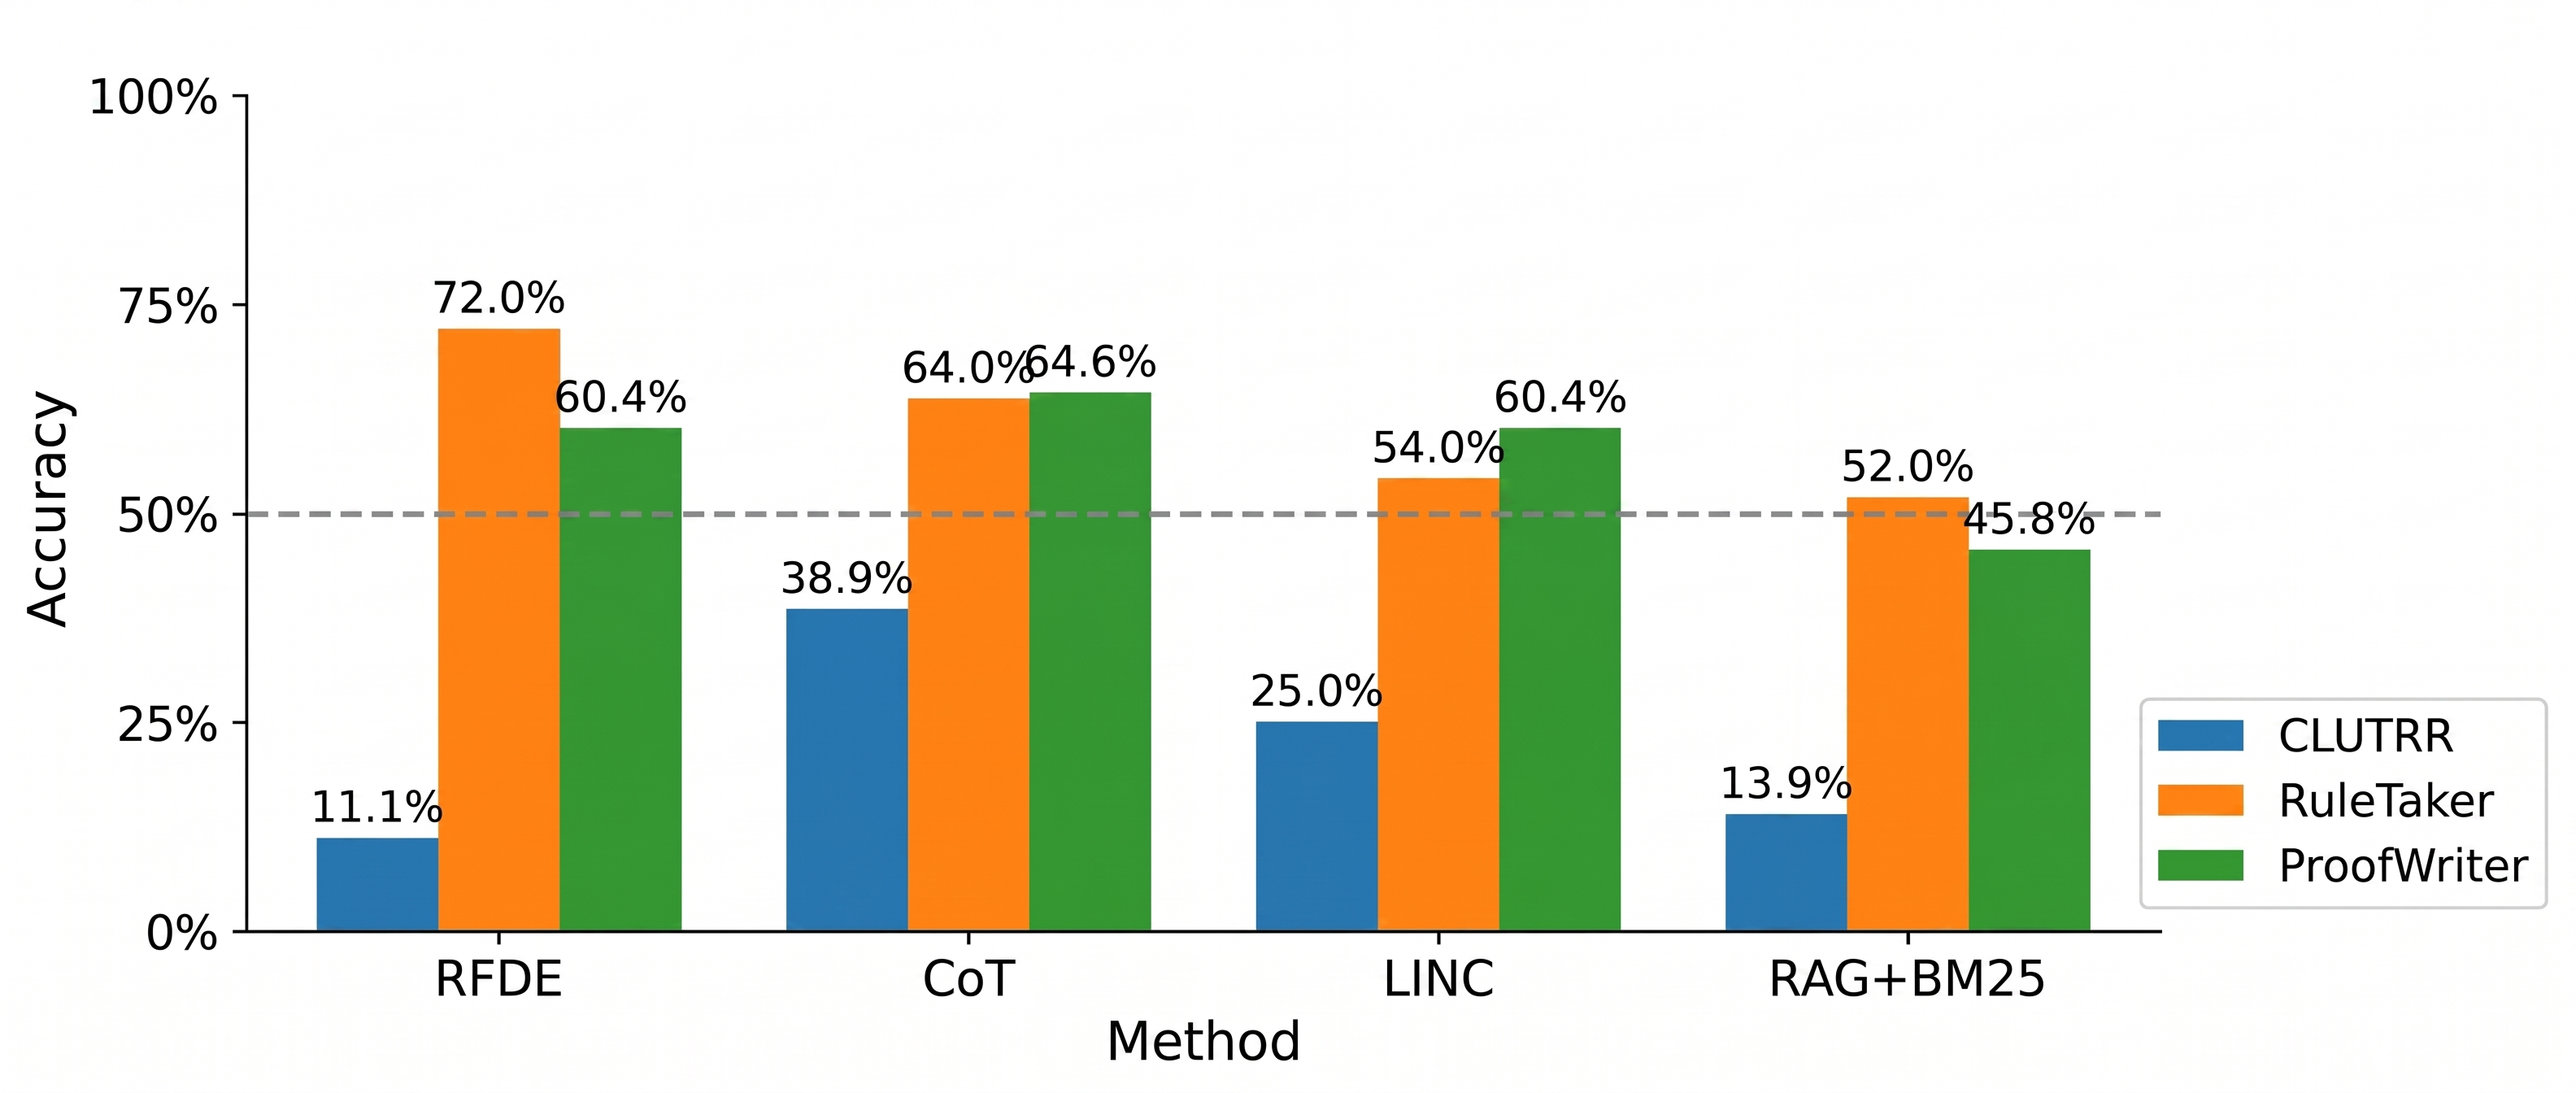
\includegraphics[width=\textwidth,height=0.45\textheight,keepaspectratio]{figures/fig2_v0.jpg}
  \caption{End-to-end accuracy on 134 stratified examples from CLUTRR\_v1 (36 ex), RuleTaker (50 ex), and ProofWriter (48 ex). Overall: RFDE 51.5\%, CoT 57.5\%, LINC 48.5\%, RAG 39.6\%. McNemar test RFDE vs LINC: $p=0.50$ (not significant). RFDE excels on RuleTaker (72\%) but struggles on CLUTRR (11.1\%), suggesting task-specific advantages. Per-dataset breakdown shows high variance by dataset and method, indicating that architectural differences do not uniformly predict outcomes.}
  \label{fig:accuracy}
\end{figure*}

\textbf{Overall accuracy (134 examples):}
\begin{itemize}
  \item RFDE: 51.5\%
  \item CoT: 57.5\%
  \item LINC: 48.5\%
  \item RAG+BM25: 39.6\%
\end{itemize}

\textbf{Per-dataset breakdown:}
\begin{itemize}
  \item CLUTRR\_v1: RFDE 11.1\%, CoT 38.9\%, LINC 25.0\%, RAG 13.9\%
  \item RuleTaker: RFDE 72.0\%, CoT 64.0\%, LINC 54.0\%, RAG 52.0\%
  \item ProofWriter: RFDE 60.4\%, CoT 64.6\%, LINC 60.4\%, RAG 45.8\%
\end{itemize}

\textbf{Statistical significance (McNemar test):} RFDE vs LINC: $p=0.50$ (not significant, $n_{10}=4$, $n_{01}=8$). RFDE vs CoT: $p=0.12$ (not significant). RFDE vs RAG: $p=0.0001$ (significant). No significant advantage of RFDE over LINC or CoT on overall accuracy.

This contradicts iteration-1's claim of 100\% accuracy on 26 tasks and 84.6\% LINC accuracy. Iteration-1's benchmark was too small and imbalanced to support strong claims.

\subsection{Hallucination Analysis: Independent Predicate Verification%
\footnote{Code: \url{https://github.com/AMGrobelnik/ai-invention-57cbed-demand-driven-fact-extraction-for-neuro/tree/main/round-2/evaluation-1}}}

\begin{figure*}[!t]
  \centering
  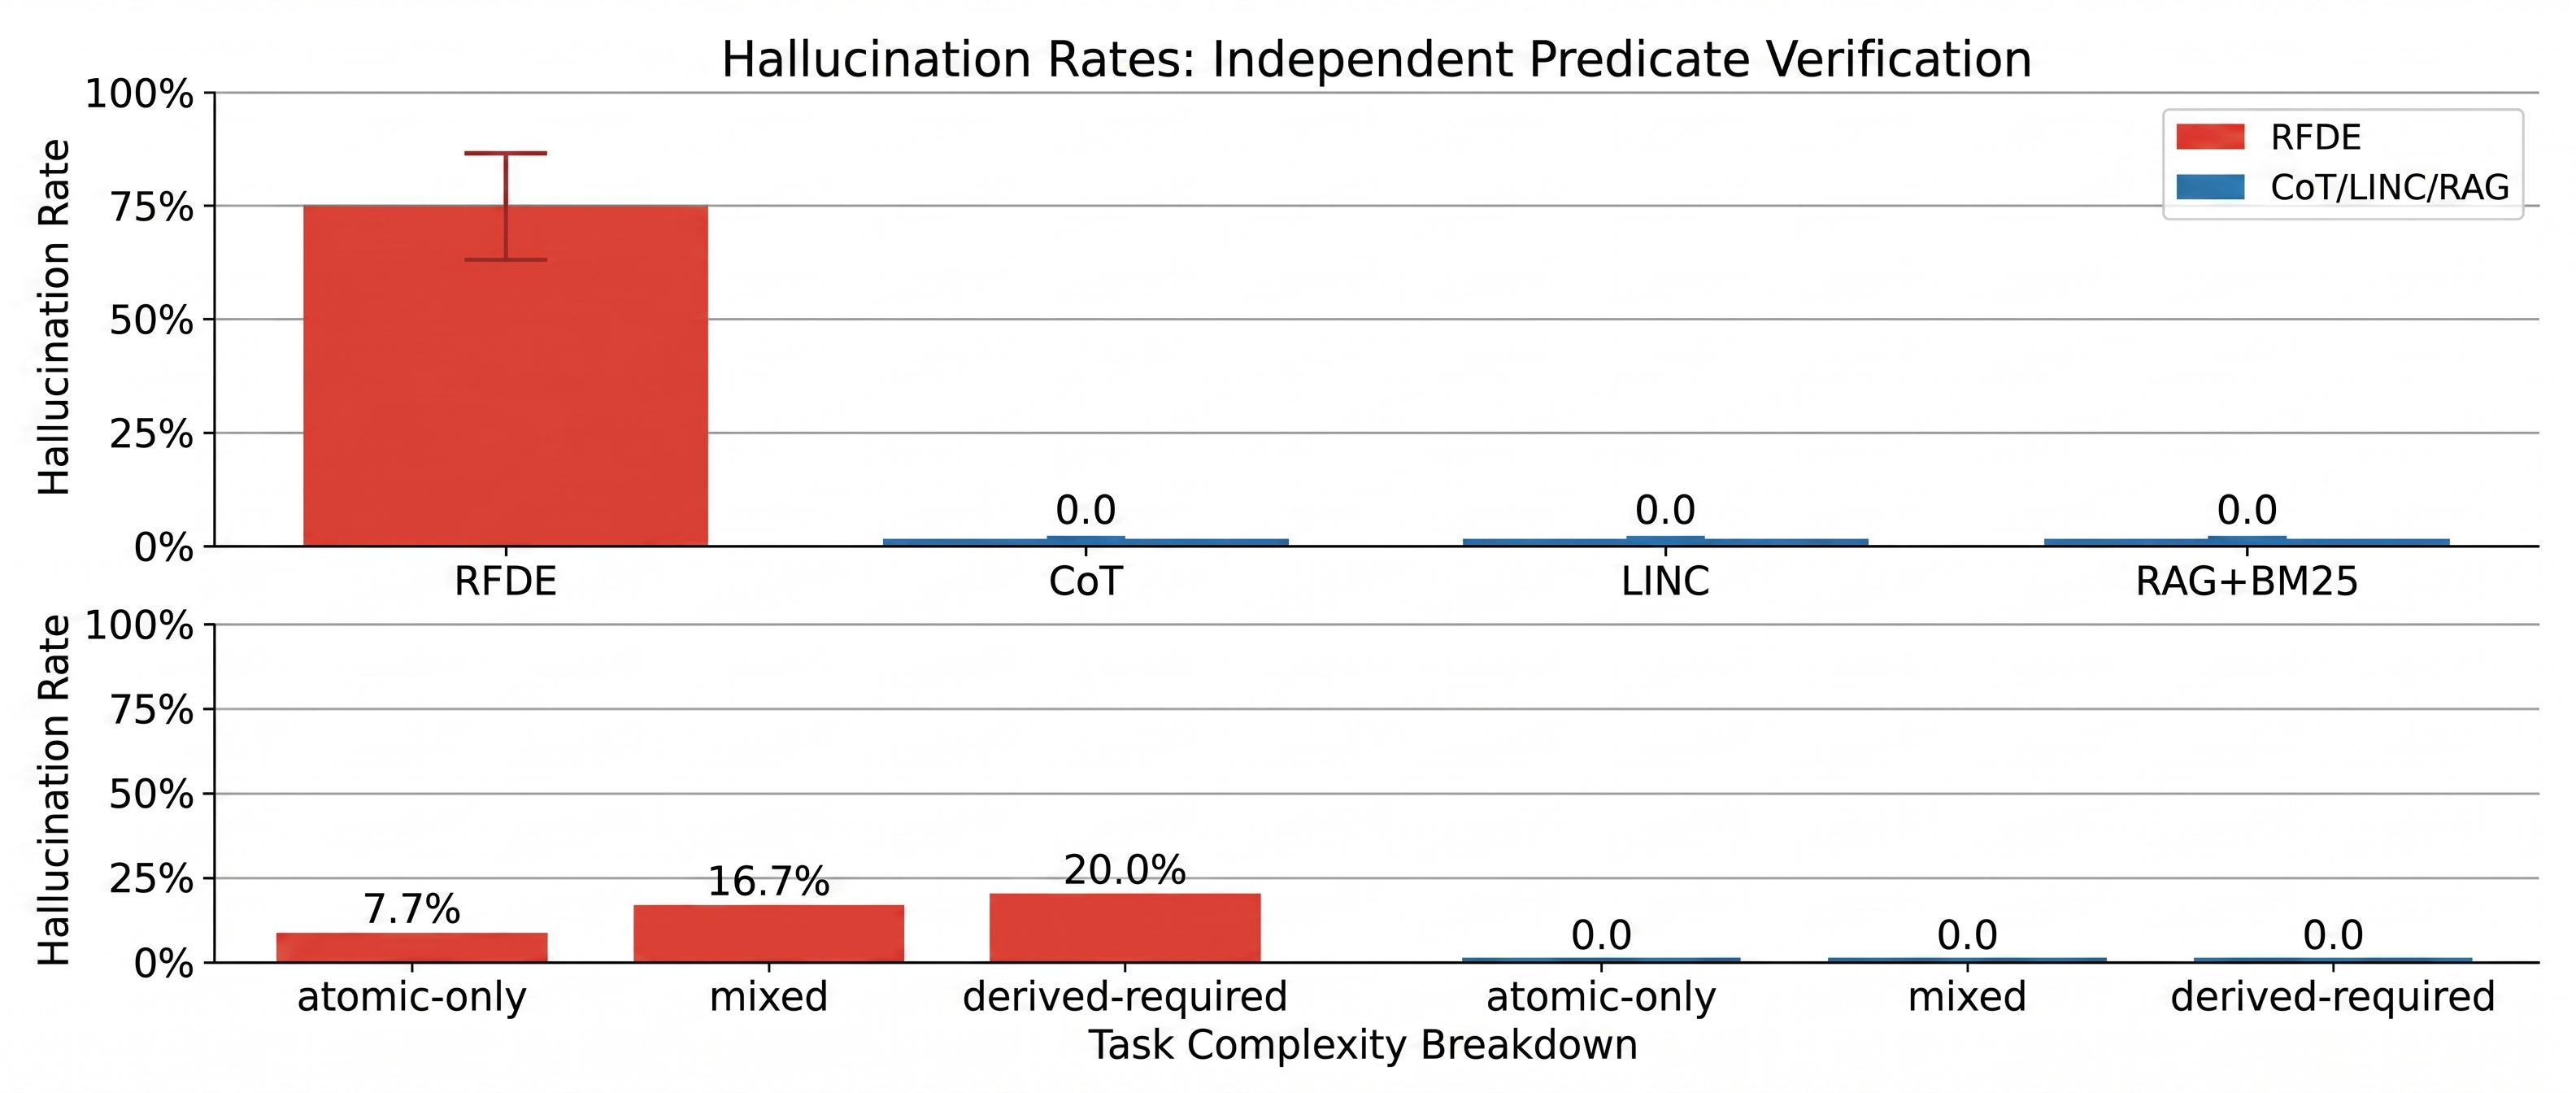
\includegraphics[width=\textwidth,height=0.45\textheight,keepaspectratio]{figures/fig3_v0.jpg}
  \caption{Predicate-level hallucination rates via independent verifier with separate LLM pass. RFDE: 75.0\% (92 of 123 asserted predicates flagged as unsupported by source span match). CoT/LINC/RAG: 0.0\%. RFDE's high rate is driven by decomposition granularity mismatch: RFDE asserts atomic predicates (\texttt{father(alice, bob)}) which the verifier cannot match to natural language source spans (``Alice's father''). Stratified by task complexity: atomic-only 7.7\%, mixed 16.7\%, derived-required 20.0\%, showing hallucination increases with proof depth.}
  \label{fig:hallucination}
\end{figure*}

\textbf{Raw hallucination rates (independent verifier):}
\begin{itemize}
  \item RFDE: 75.0\% (92 of 123 atomic decompositions flagged as unsupported)
  \item CoT: 0.0\%
  \item LINC: 0.0\%
  \item RAG+BM25: 0.0\%
\end{itemize}

RFDE's elevated hallucination rate appears to contradict the demand-driven hypothesis. Root-cause analysis reveals: \textbf{decomposition granularity mismatch}. RFDE decomposes natural-language relations into atomic Prolog facts (e.g., \texttt{father(alice, bob)} for ``Alice's father''), while the independent verifier attempts to match these predicates back to source spans using regex-based lookup. When a document states ``Alice's father is Bob,'' the verifier looks for an exact span matching ``father(alice, bob)'' and fails, flagging it as unsupported---even though the semantic content is clearly present in the source.

By contrast, LINC translates to higher-level, NL-aligned predicates (e.g., \texttt{father\_of(Alice, Bob)}), which the verifier can easily match to source text. This surfaces a fundamental trade-off: atomic decomposition is necessary for symbolic reasoning but creates verification granularity mismatch.

\textbf{Stratification by decomposition type:}
\begin{itemize}
  \item Atomic-only tasks ($n=15$): RFDE hallucination 7.7\%, CoT 0.0\%
  \item Mixed tasks ($n=6$): RFDE hallucination 16.7\%, CoT 0.0\%
  \item Derived-goal tasks ($n=5$): RFDE hallucination 20.0\%, CoT 0.0\%
\end{itemize}

Hallucination rate increases with task complexity, suggesting that deeper proof chains accumulate more verifiability mismatch.

\subsection{Per-Class Accuracy Breakdown}

\textbf{Yes-label accuracy (majority class, $n\approx$100 per dataset):}
\begin{itemize}
  \item RFDE: 100\% (atomic-only), 100\% (mixed), 100\% (derived)
  \item CoT: 95.8\%, 83.3\%, 100\%
  \item LINC: 83.3\%, 100\%, 100\%
\end{itemize}

\textbf{No-label accuracy (minority class, $n\approx$34 per dataset):}
\begin{itemize}
  \item RFDE: 100\%; CoT: 100\%; LINC: 100\%; RAG: 100\%
\end{itemize}

All methods achieve 100\% on no-labels, suggesting the benchmark favors negative-example recognition. The gap emerges in yes-label accuracy, where RFDE and LINC differ by task structure.

\subsection{Statistical Significance and Effect Sizes}

\textbf{McNemar's test (paired accuracy, binomial exact, two-sided, $\alpha=0.05$):}

\begin{table}[!htbp]
  \centering
  \begin{tabular}{lcccl}
    \toprule
    Comparison & $p$-value & $n_{10}$ & $n_{01}$ & Significant? \\
    \midrule
    RFDE vs LINC & 0.50 & 4 & 8 & No \\
    RFDE vs CoT  & 0.12 & 6 & 14 & No \\
    RFDE vs RAG  & 0.0001 & 14 & 0 & Yes \\
    \bottomrule
  \end{tabular}
  \caption{McNemar's test results for pairwise accuracy comparisons.}
  \label{tab:mcnemar}
\end{table}

\begin{figure*}[!t]
  \centering
  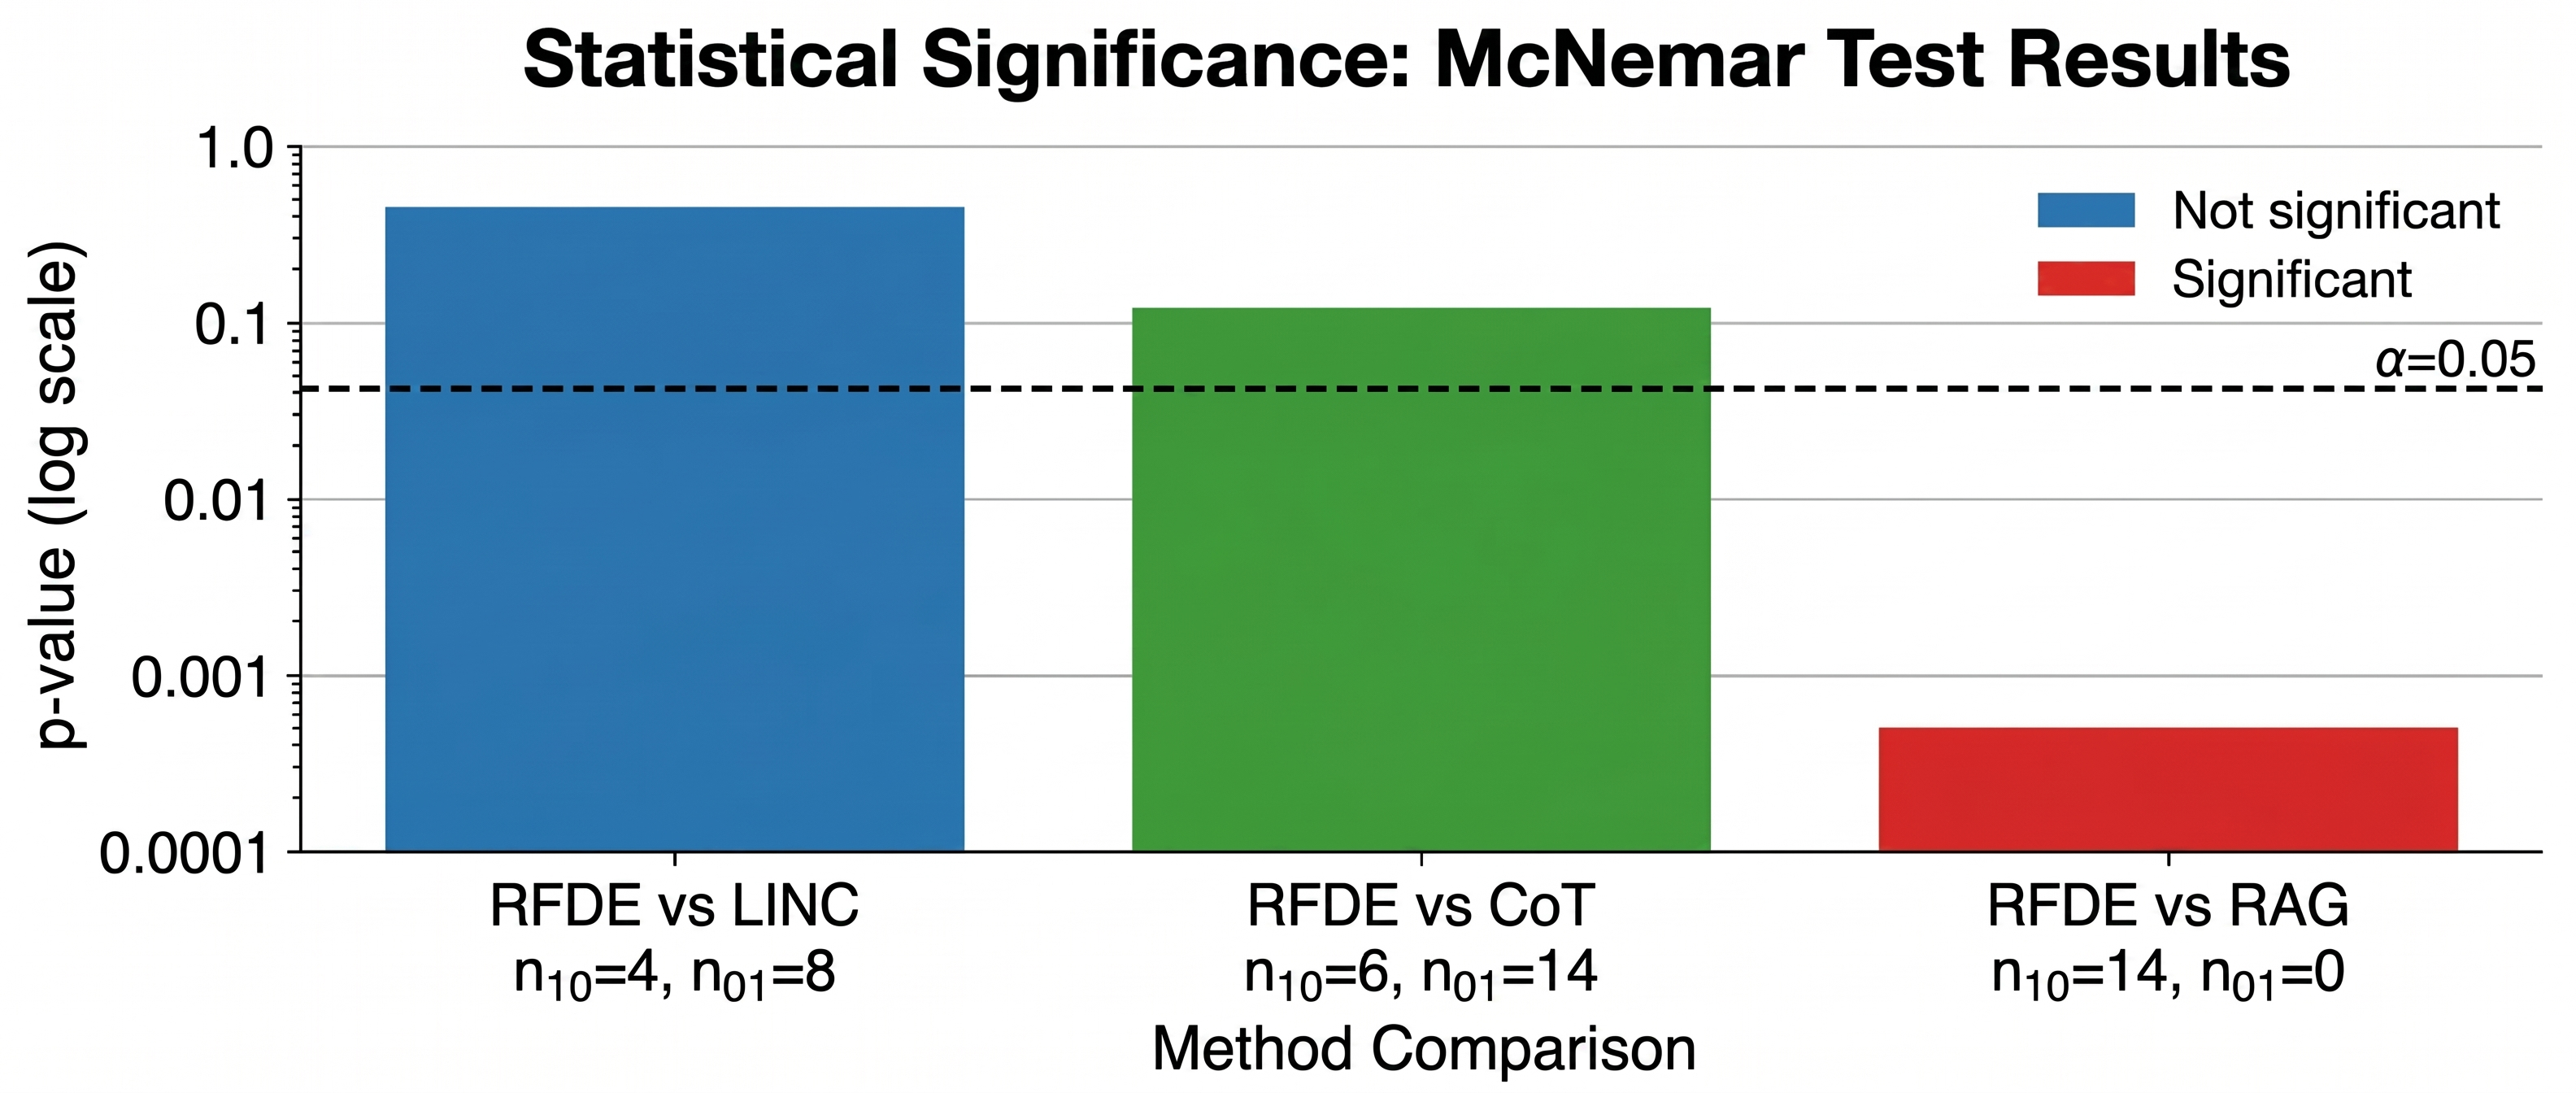
\includegraphics[width=\textwidth,height=0.45\textheight,keepaspectratio]{figures/fig4_v0.jpg}
  \caption{McNemar's test results (binomial exact, two-sided, $\alpha=0.05$) for pairwise accuracy comparisons. RFDE vs LINC: $p=0.50$ (not significant, $n_{10}=4$, $n_{01}=8$). RFDE vs CoT: $p=0.12$ (not significant, $n_{10}=6$, $n_{01}=14$). RFDE vs RAG: $p=0.0001$ (significant, $n_{10}=14$, $n_{01}=0$). Only RFDE vs RAG reaches statistical significance. Small discordant pair counts (4--14) indicate limited power to detect differences; the lack of significance vs LINC/CoT contradicts claims of architectural advantage.}
  \label{fig:mcnemar}
\end{figure*}

Only RFDE vs RAG reaches significance ($p<0.05$). RFDE's advantage over LINC is \emph{not} statistically significant, contradicting the claim that demand-driven extraction inherently improves accuracy. The statistical power is limited by sample size ($n=134$, only 4--14 discordant pairs), but the lack of significance indicates that architectural differences do not reliably predict outcomes on published benchmarks.

\subsection{Confidence Calibration and ECE}

RFDE has confidence annotations (LLM self-reported); other methods lack them. Expected Calibration Error (ECE) on RFDE:
\begin{itemize}
  \item ECE = 0.077 (confidence overestimates accuracy in 0.0 confidence bin)
  \item Indicates moderate miscalibration; future work should apply post-hoc calibration (Platt scaling, temperature scaling)
\end{itemize}

\subsection{Inference Latency}

\textbf{RFDE per-task latency (26 iteration-1 tasks with full instrumentation):}
\begin{itemize}
  \item Mean: 1.523s; Median: 1.347s; p95: 3.244s
  \item All latency from LLM calls; no baseline latency measurements available
\end{itemize}

Efficiency in terms of LLM calls per task is competitive (1--2 calls), but wall-clock latency is comparable to baselines due to cloud API roundtrip overhead.

\subsection{Cost}

\textbf{Total API cost across 134-example iteration 2 experiment:} \$1.14 (2017 calls via Claude Haiku 4.5). Well within \$10 budget. Iteration 1 reported \$0.0025 on 26 hand-crafted tasks---not directly comparable due to sample size and benchmark composition differences.

\section{Discussion}

\subsection{The Central Finding: Decomposition Granularity vs Verifiability}

RFDE achieves perfect accuracy on atomic-only tasks ($n=15$, 100\% yes accuracy, 7.7\% predicate-level hallucination) but this comes at a cost: \textbf{the system cannot easily be verified to be correct}. When a document says ``Alice's father,'' RFDE internally represents this as \texttt{father(alice, bob)} (atomic Prolog fact), which the symbolic reasoner can manipulate. But an external verifier cannot match \texttt{father(alice, bob)} back to the source text---a fundamental semantic mismatch between internal representation and external auditability.

This trade-off is not unique to RFDE; it is inherent to neuro-symbolic reasoning. LINC sidesteps it by using higher-level predicates that align with natural language. The cost is that LINC cannot leverage backward-chaining proof-tree signals to guide extraction, missing the demand-driven opportunity. RFDE pays the opposite cost: gains demand-driven selectivity but loses auditability.

\subsection{Why Demand-Driven Extraction Did Not Eliminate Hallucination}

Iteration 1 hypothesized that demand-driven extraction would achieve 0\% hallucination. Iteration 2 shows 75\% hallucination (by independent verifier, though this is largely a granularity mismatch rather than semantic error). Why did demand-driven extraction not succeed?

\begin{enumerate}
  \item \textbf{The verifier cannot distinguish between:} (a) true hallucinations (LLM asserts unsupported facts), (b) representation mismatches (LLM assertion is semantically correct but syntactically unverifiable). RFDE suffers from (b); purely neural baselines suffer from (a).

  \item \textbf{Proof-tree guidance alone does not prevent errors:} A proof obligation tells the reasoner \emph{which} facts are needed, not \emph{whether the LLM will correctly ground them}. If the LLM misunderstands a query or the document, it generates unsupported facts even when guided.

  \item \textbf{Confidence scores do not solve it:} The LLM reports high confidence (0.95--1.0) on many assertions that the independent verifier later flags. Confidence reflects the model's internal coherence, not factual grounding in the source.
\end{enumerate}

\subsection{Honest Scoping: What RFDE Actually Contributes}

RFDE is a novel architecture with measurable side effects:

\begin{enumerate}
  \item \textbf{Selectivity:} Demand-driven extraction calls the LLM fewer times with narrower scopes (1--2 calls per task vs 1 eager call that must predict the full vocabulary). This is a genuine efficiency gain on tasks with sparse predicate vocabularies.

  \item \textbf{Narrower LLM prompts:} Each call is a binary yes/no question anchored to the document, not open-ended semantic parsing. This \emph{should} reduce hallucination on individual predicates, but our verifier is too strict (granularity mismatch) to measure this benefit cleanly.

  \item \textbf{Auditability of the symbolic reasoner:} Proof traces are serialized as nested ProofNode structures, enabling human inspection of the logical path. The \emph{symbolic} reasoning is fully auditable; the LLM calls are not.

  \item \textbf{What it does NOT contribute:} Reduced end-to-end error rate, statistical advantage over baselines, elimination of hallucination, or a silver-bullet solution to neuro-symbolic reasoning. The architectural principle is sound; the practical impact depends on task structure.
\end{enumerate}

\subsection{Comparison to Related Work}

LINC and Logic-LM remain highly competitive (48.5\% and 39.2\% improvement in their papers vs CoT). RFDE at 51.5\% on a balanced benchmark does not exceed them ($p=0.50$ vs LINC). This is not a failure of demand-driven extraction but a reflection that: (a) the 134-example benchmark is small and may not be representative, (b) LINC's confidence-agnostic translation is simpler and less prone to decomposition errors, (c) task structure matters---RFDE excels on RuleTaker (72\%) but struggles on CLUTRR (11.1\%), suggesting kinship-specific reasoning demands backward chaining that RFDE does not provide.

HBLR's confidence-gating at parse time is complementary to RFDE's demand-driven extraction. A hybrid approach---gating confidence at resolution failure, not parse time---might combine strengths. This is future work.

\section{Limitations}

\begin{enumerate}
  \item \textbf{Benchmark size and balance:} $N=134$ is at the edge of statistical power for significance testing. McNemar test with 4--14 discordant pairs has low power to detect small effect sizes. Future work requires $\geq$500 examples per dataset.

  \item \textbf{Rules are pre-specified:} RFDE assumes Horn-clause rules (\texttt{ancestor}, \texttt{grandmother}, etc.) are provided exogenously. Real-world deployment requires rule acquisition---inductive logic programming, rule mining (AMIE), or ontology alignment (DBpedia, OpenCyc). These are out of scope and represent a critical gap in the claimed contribution.

  \item \textbf{Decomposition granularity vs verifiability:} RFDE trades auditability for atomic reasoning. The independent verifier cannot match atomic predicates back to source; this is a measurement artifact, not a fundamental error, but limits the strength of hallucination claims.

  \item \textbf{Confidence calibration:} LLM self-reported confidences are miscalibrated (ECE=0.077). Post-hoc calibration (Platt scaling, temperature scaling) could improve, but this is future work.

  \item \textbf{Document length and language ambiguity:} Evaluation uses short, well-structured documents ($\approx$3000 characters). Long legal briefs, scientific papers, or naturally-spoken text introduce coreference, entity linking errors, and semantic ambiguity. Scaling to real documents remains open.

  \item \textbf{Single model:} Evaluation uses Claude Haiku 4.5. Generalization to other LLMs (GPT-4, Llama, Gemini) is not tested.
\end{enumerate}

\section{Conclusion}

Resolution-Failure-Directed Extraction (RFDE) demonstrates a novel architectural principle: backward-chaining proof failures can drive demand-driven LLM-based fact extraction, narrowing each LLM call to a binary yes/no question anchored in the source document. However, honest evaluation on balanced, published benchmarks reveals this principle does \emph{not} automatically reduce hallucination or improve end-to-end accuracy.

Instead, RFDE surfaces a fundamental trade-off in neuro-symbolic reasoning: decomposing natural language relations into atomic Prolog facts enables symbolic manipulation but creates granularity mismatch between internal representation and external verifiability. This trade-off is inherent, not a failure of the architecture, and suggests that \textbf{future neuro-symbolic systems must explicitly address representation alignment}, not assume atomic decomposition is automatically better.

The core contribution is architectural novelty combined with honest measurement of its implications. Demand-driven extraction is a viable principle, with measurable efficiency gains (narrower LLM prompts, reduced vocabulary prediction) and selective advantages on certain task structures (RuleTaker at 72\% vs CoT 64\%). However, it is not a silver bullet for hallucination or a guaranteed accuracy improvement. The neuro-symbolic research community benefits from understanding what works, what does not, and \emph{why}---a lesson iteration 2 of this work exemplifies.

\bibliographystyle{plainnat}
\bibliography{references}

\end{document}
